In previous sections, we propose a Multistream Domain Adaptation (MSDA) framework to address major issues in our problem setting. 
To be specific, the assumption of heterogeneous domain holds valid between source and target streams,
while there are concept drift in both streams as well. Thus, our goal of designing this framework is to use as much information as possible from the source stream,
to predict the instance labels in the target stream.

To achieve this goal, we establish a framework with the following modules:

1. A feature space mapping module that helps find an optimized latent subspace for both source and target streams. 

2. A concept drift detection module that detect concept drift in both source and target streams.

\begin{figure}[t]
\centering
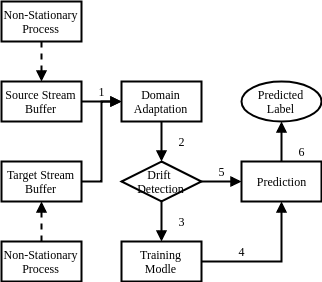
\includegraphics[width=1.0\columnwidth]{Figures/flowchart.png}
\caption{Flowchart}
\label{fig:flowchart}
\end{figure}

Applying both those two modules altogether, once a concept drift is detected, we use data instances from both in the most recent window to update the feature mapping, so that the domain adaptation problem can be addressed. The flowchart of this algorithm can be found in Figure \ref{fig:flowchart}.

In our framework, data instances are generated simultaneously from both source and target domains. 
At first, a domain adaptation module is triggered to learn projection functions for both source and target data instances (step 1). 
New arriving instances are transformed to latent feature representation accordingly. Next, the change point detection module detects if there is a significant change in both source and target streams within the sliding windows. 
Once a change point is detected, new projection functions of buffer $B_s$ from source stream and $B_t$ from target stream. 
New classifiers are trained as well based on these two buffers. Finally, newly updated classifiers are used to  predict the labels of adapted data instances from target stream $T$. Details of our proposed method is proposed as follows.

\begin{algorithm}[h]  
\caption{MSDA Algorithm}  
\label{alg::overall}  
\begin{algorithmic}[1]  
\Require  
Labeled source stream $S$,
Unlabeled target stream $T$,  
The size of sliding window $k$.
Similarity parameter $\beta$.
\Ensure  
Labels predicted on $T$.
\While {$S$ or $T$ $exists$}
\State $B_s, B_t \gets readData(S,T)$
\State \# Domain Adaptation
\State $W_s, W_t \gets genProjectionFunction(B_s, B_t, \beta)$
\State $L_s, L_t \gets genProjectionMatrix(B_s, B_t, W_s, W_t)$
\State \# Concept drift detection and correction
\State Calculate initial $Disc_s, Disc_t$
\If {$z \gets checkDrift(Disc_s)$}
\State $B_s, Disc_s \gets updateBuffer$$(z, B_s, W_s)$
\State $M \gets buildModel(B_s)$
\EndIf
%\State $W_t, \hat{Y} \gets preData(E_{param}, B_t)$
\If {$z \gets checkDrift(Disc_t)$}
\State $B_t, W_t \gets updateBuffer$$(z, B_t, Disc_t)$
\State $M \gets buildModel(B_s, B_t)$
% \State $M \gets buildSourceModel(B_t)$
\EndIf
\State \# Generate predictions
\State $\hat{y_{t}} \gets getPrediction(M,B_s, B_{t})$
% \State print $getMAE (\hat{y}_t, B_t)$
\EndWhile

\end{algorithmic}  
\end{algorithm}

\subsection{Initialization and Domain Adaptation}

In our proposed framework of MSDA, instances from source and target streams are stored in $B_{s}$ and $B_{t}$ respectively. 
Recalling our problem setting, data in $B_{s}$ have true labels, while data in $B_t$ come without true labels. 
Also, for computational purposes, we design our approach in a way that buffer size in both source and target streams are the same, which means the numbers of data instances in processing window for source and target streams are identical. 
Thus, given a certain time $t$, data that we have are: source stream window matrix $B_s \in \mathds{R}^{m\times k}$; source stream window labels vector $Y_{s} \in \mathds{R}^{1 \times k}$, and; target stream window matrix $B_t \in \mathds{R}^{n \times k}$. 
In this case, the best projection strategy of $L_{s}$ and $L_{t}$ in the latent feature space would be the minimization of following objective function:
\begin{equation}
\label{fcn:overallMinimization}
    \min_{L_{s}, L{t}}\ell\left ( B_s, L_{s} \right ) + \ell\left ( B_t, L_{t} \right ) + \beta \mathbf{D}\left(L_{s}, L_{t} \right )
\end{equation}
where $\ell\left(\cdot , \cdot \right)$ is a distortion function that evaluates the differences between original data and projected data (e.g., $S$ and $L_{s}$). 
$\mathbf{D}\left(\cdot, \cdot\right)$ is the co-regularizer that promotes the similarities between the two projected domains ($L_{s}$ and $L{t}$). $\beta$ is a parameter that determines how desirable the two projected data are similar. 
Equation \ref{fcn:overallMinimization} is further analyzed as follows. 
The first two terms are expected to preserve the structure of the original data as much as possible. 
Therefore, we define the loss function $\ell\left(\cdot, \cdot\right)$ as the Frobenius norm, which can also be expressed as matrix trace norm:
\begin{equation}
\begin{split}
\label{fcn:norm}
    \ell\left(B_s, L_{s}\right) + \ell\left(B_t, L_{t}\right) = \left \| B_s - L_{s}W_{s}  \right \|_{F}^2 \\
    + \left \| B_t - L_{t}W_{t}\right \|_{F}^2 
\end{split}
\end{equation}
in which we factorize the original data into projections ($L_{s}$ and $L_{t}$) by linear mapping functions ($W_{s}$ and $W_{t}$).
Also, note that here we are not applying the alternative definition such as $\ell\left(B_s,L_{s}\right) $ as $\left \| B_{s}W_{s} - L_{s}  \right \|_{F}^2$, since this definition will always lead to a trivial solution $W_{s} = 0$ and $L_{s} = 0$, thus $B_{s}W_{s} = L_{s} = 0$ will always minimize the objective function. By the equation described above, the projected data should preserve the structures of original data.

Furthermore, we define $\mathbf{D}\left(L{s}, L_{t}\right)$ as follows:
\begin{equation}
\label{fcn:crossSimilarity}
    \mathbf{D}\left(L_{s}, L_{t}\right) =\frac{1}{2}\left(\ell\left(B_s, L_{t}\right) + \ell\left(B_t, L_{s}\right)\right)
\end{equation}
which is the mean value of cross-similarity between the original data and projected data. Combined with the parameter $\beta$, which controls the trade-off of importance of semantic similarity co-regularization by minimizing the differences between $\mathbf{D}(L_{s}, L_{t})$.

Combine Equation \ref{fcn:overallMinimization}, \ref{fcn:norm} and \ref{fcn:crossSimilarity} together, we can obtain the overall optimization objective function as follows:
\begin{equation}
\label{fcn:finalObjectiveFunction}
\begin{split}
    \mathcal{O} = \left \| B_s - L_{s}W_{s}  \right \|_{F}^2 + \left \| B_t - L_{t}W_{t}\right \|_{F}^2 \\
    + \frac{1}{2}\beta \left(\ell\left(B_s, L_{t}\right) + \ell\left(B_t, L_{s}\right)\right)
\end{split}
\end{equation}
Notice here the projection itself will perform rotation, scaling on the target matrix to minimize the difference.
Since $L_s$ and $L_t$ are orthogonal matrix, $B_{s}^{\intercal}B_{s}=1$. Also, we are applying the cyclic permutation property of trace:
\begin{equation}
    \textbf{tr}\left(W_{t}^{\intercal}L_{t}^{\intercal}B_{t}\right) = \textbf{tr}\left(L_{t}^{\intercal}B_{t}W_{t}^{\intercal}\right)
\end{equation}

Thus, Equation \ref{fcn:finalObjectiveFunction} can be expanded by the representation of trace.

We therefore adopt an alternative formula to solve this problem by iterative fixing one of the projection matrices until the remaining one converge. 
That is, we can take the derivative of $\mathcal{O}$ with regard to $W_s$ and $W_t$.
Under this conditions, our formula is defined as follows accordingly.

\begin{equation}
\begin{split}
    \frac{\partial \mathcal{O}}{\partial W_{t}} = -2L_{t}^{\intercal} - \beta L_{s}^{\intercal}B_{t} + (2+\beta)W_{t} \\
    \frac{\partial \mathcal{O}}{\partial W_{s}} = -2L_{s}^{\intercal} - \beta L_{t}^{\intercal}B_{t} + (2+\beta)W_{s}
\end{split}
\end{equation}

According to~\cite{long2008general}, we know that setting both partial derivatives would generate the optimal solution based on KKT conditions.
Consequently, the projection function for both source and target stream can be formulated as:

\begin{equation}
\begin{split}
    W_s = \cfrac{1}{2+\beta}\left(2 L_{s}^\intercal B_{s} + \beta L_{t}^\intercal B_{s}\right) \\
    W_t = \cfrac{1}{2+\beta}\left(2 L_{t}^\intercal B_{t} + \beta L_{s}^\intercal B_{t}\right) \\
\end{split}
\end{equation}

After steps described above, the optimal projection for both source and target stream to the latent feature space would be formed accordingly. 

% Furthermore, we need to screen the optimization to avoid mappings between two totally unrelated data. A sample selection algorithm is used to eliminate those unrelated examp/les, that is, if the source data is too different from target data, we will consider that it is ``too risky'' to conduct the domain adaptation.

%%%%%%%%%%%%%%%%%%%%%%%%%%%%%%%%%%%%%%%%%%%
% Here goes Tao's code
%%%%%%%%%%%%%%%%%%%%%%%%%%%%%%%%%%%%%%%%%%%

\subsection{Classification Module}
Initially, we train a classifier using a small set of data instances from both $S$ and $T$, which are referred to as the warm-up period data. Here, we learn a $K\times K'$ projection matrix $\mathbf{P}$ to overcome joint distribution difference between the two streams. The new data representation is obtained by the JDM using warm-up period data from $\mathcal{W}_S$ and $\mathcal{W}_T$ as follows:
\begin{equation}
\begin{cases}
\mathcal{W}_{newS}^{(i)}=\mathbf{P}^T\mathcal{W}_S^{(i)}, \qquad \mathcal{W}_S^{(i)}\in \mathcal{W}_S \\
\mathcal{W}_{newT}^{(j)}=\mathbf{P}^T\mathcal{W}_T^{(j)}, \qquad \mathcal{W}_T^{(j)}\in \mathcal{W}_T\\
\end{cases}
\end{equation}

Any learning algorithm can be used in COMC. As new instances arrive in $S$ or $T$, the classifier is updated if there is a drift to ensure that it represents the current concepts. A new base model is trained using data in $\mathcal{W}_S$ and $\mathcal{W}_T$ at that time. Drift detection and the updating method used by COMC will be discussed later in this section. COMC predicts the  class label of an incoming test instance from the target stream after projecting the instance into the new data format.


\subsection{Change Detection Module (CDM)}

\subsection{Complexity Analysis}